\chapter{Autoencoders}
\label{chap-autoencoders}

In previous chapters, we have largely focused on classification and
regression problems, where we use supervised learning with training
samples that have both features/inputs and corresponding outputs or labels, to
learn hypotheses or models that can then be used to predict labels for
new data.

In contrast to supervised learning paradigm, we can also have an unsupervised learning setting, where we only have features but no
corresponding outputs or labels for our dataset. On natural question aries then: if there are no labels, what are we learning?

%% One canonical example of unsupervised learning is clustering, where
%% the goal is to develop algorithms that can reason about ``similarity''
%% among data points's features, and group the data points into
%% clusters. We will learn about clustering towards the end of the
%% semester in Chapter~\ref{chap-clustering}.

One canonical example of unsupervised learning is clustering,
which we learned about in Chapter~\ref{chap-clustering}.
In clustering, the goal is to develop algorithms that can reason about
``similarity'' among data points's features, and group the data points
into clusters.

  {\em Autoencoders}\index{autoencoder} are another family of unsupervised learning
algorithms, in this case seeking to obtain insights about our data by
learning compressed versions of the original data, or, in other words,
by finding a good lower-dimensional feature representations of the
same data set. Such insights might help us to discover and
characterize underlying factors of variation in data, which can aid in
scientific discovery; to compress data for efficient storage or
communication; or to pre-process our data prior to supervised
learning, perhaps to reduce the amount of data that is needed to learn
a good classifier or regressor.

\section{Autoencoder structure}

Assume that we have input data $\mathcal{D} = \{x^{(1)}, \ldots,
  x^{(n)} \}$, where $x^{(i)}\in \mathbb{R}^d$. We seek to learn an
autoencoder that will output a new dataset $\mathcal{D}_{out} =
  \{a^{(1)}, \ldots, a^{(n)}\}$, where $a^{(i)}\in \mathbb{R}^k$ with $k
  < d$. We can think about $a^{(i)}$ as the new \textit{representation}
of data point $x^{(i)}$. For example, in Fig.~\ref{fig:illustration}
we show the learned representations of a dataset of MNIST digits with
$k=2$. We see, after inspecting the individual data points, that
unsupervised learning has found a compressed (or {\em latent}\index{latent representation})
representation where images of the same digit are close to each
other, potentially greatly aiding subsequent clustering or
classification tasks.

\begin{figure}[h!]
  \centering
  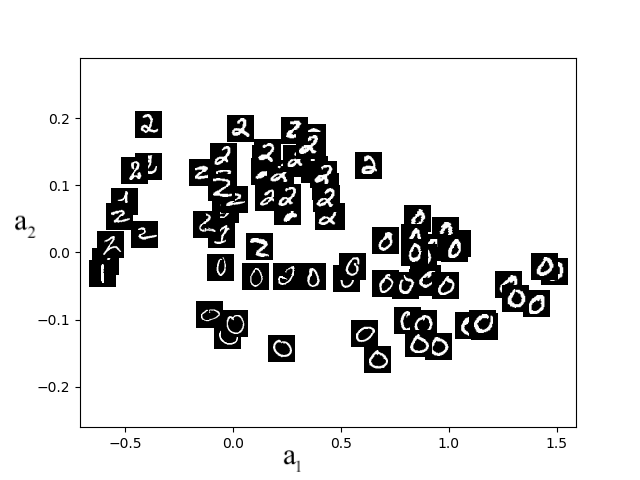
\includegraphics[width= .5\textwidth]{figures/autoencoder_mnist.png}
  \caption{\small Compression of digits dataset into two
    dimensions. The input $x^{(i)}$, an image of a handwritten
    digit, is shown at the new low-dimensional representation
    $(a_1,a_2)$.}
  \label{fig:illustration}
\end{figure}

Formally, an autoencoder consists of two functions, a vector-valued
\textit{encoder} $g : \mathbb{R}^d \rightarrow \mathbb{R}^k$ that
deterministically maps the data to the representation space $a \in
  \mathbb{R}^k$, and a \textit{decoder} $h : \mathbb{R}^k \rightarrow
  \mathbb{R}^d$ that maps the representation space back into the
original data space.

In general, the encoder and decoder functions might be any functions
appropriate to the domain. Here, we are particularly interested in
neural network embodiments of encoders and decoders.
The basic architecture of one such autoencoder, consisting of only a single
layer neural network in each of the encoder and decoder, is shown in
Figure~\ref{fig:autoencoder}; note that bias terms $W^1_0$ and $W^2_0$ into
the summation nodes exist, but are omitted for clarity in the figure.
In this example, the original
$d$-dimensional input is compressed into $k=3$ dimensions via the
encoder $g(x; W^1, W^1_0)=f_1(W{^1}^T x + W^1_0)$ with $W^1 \in
  \mathbb{R}^{d \times k}$ and $W^1_0 \in \mathbb{R}^k$,
and where the non-linearity $f_1$ is applied to each
dimension of the vector. To recover (an approximation to) the
original instance, we then apply the decoder $h(a; W^2, W^2_0) = f_2(W{^2}^T
  a + W^2_0)$, where $f_2$ denotes a different non-linearity (activation
function). In general, both the decoder and the encoder could involve
multiple layers, as opposed to the single layer shown here. Learning
seeks parameters $W^1, W^1_0$ and $W^2, W^2_0$ such that the reconstructed
instances, $h(g(x^{(i)}; W^{1}, W^1_0); W^{2}, W^2_0)$, are close to the original
input $x^{(i)}$.

\begin{figure}[h]
  \centering
  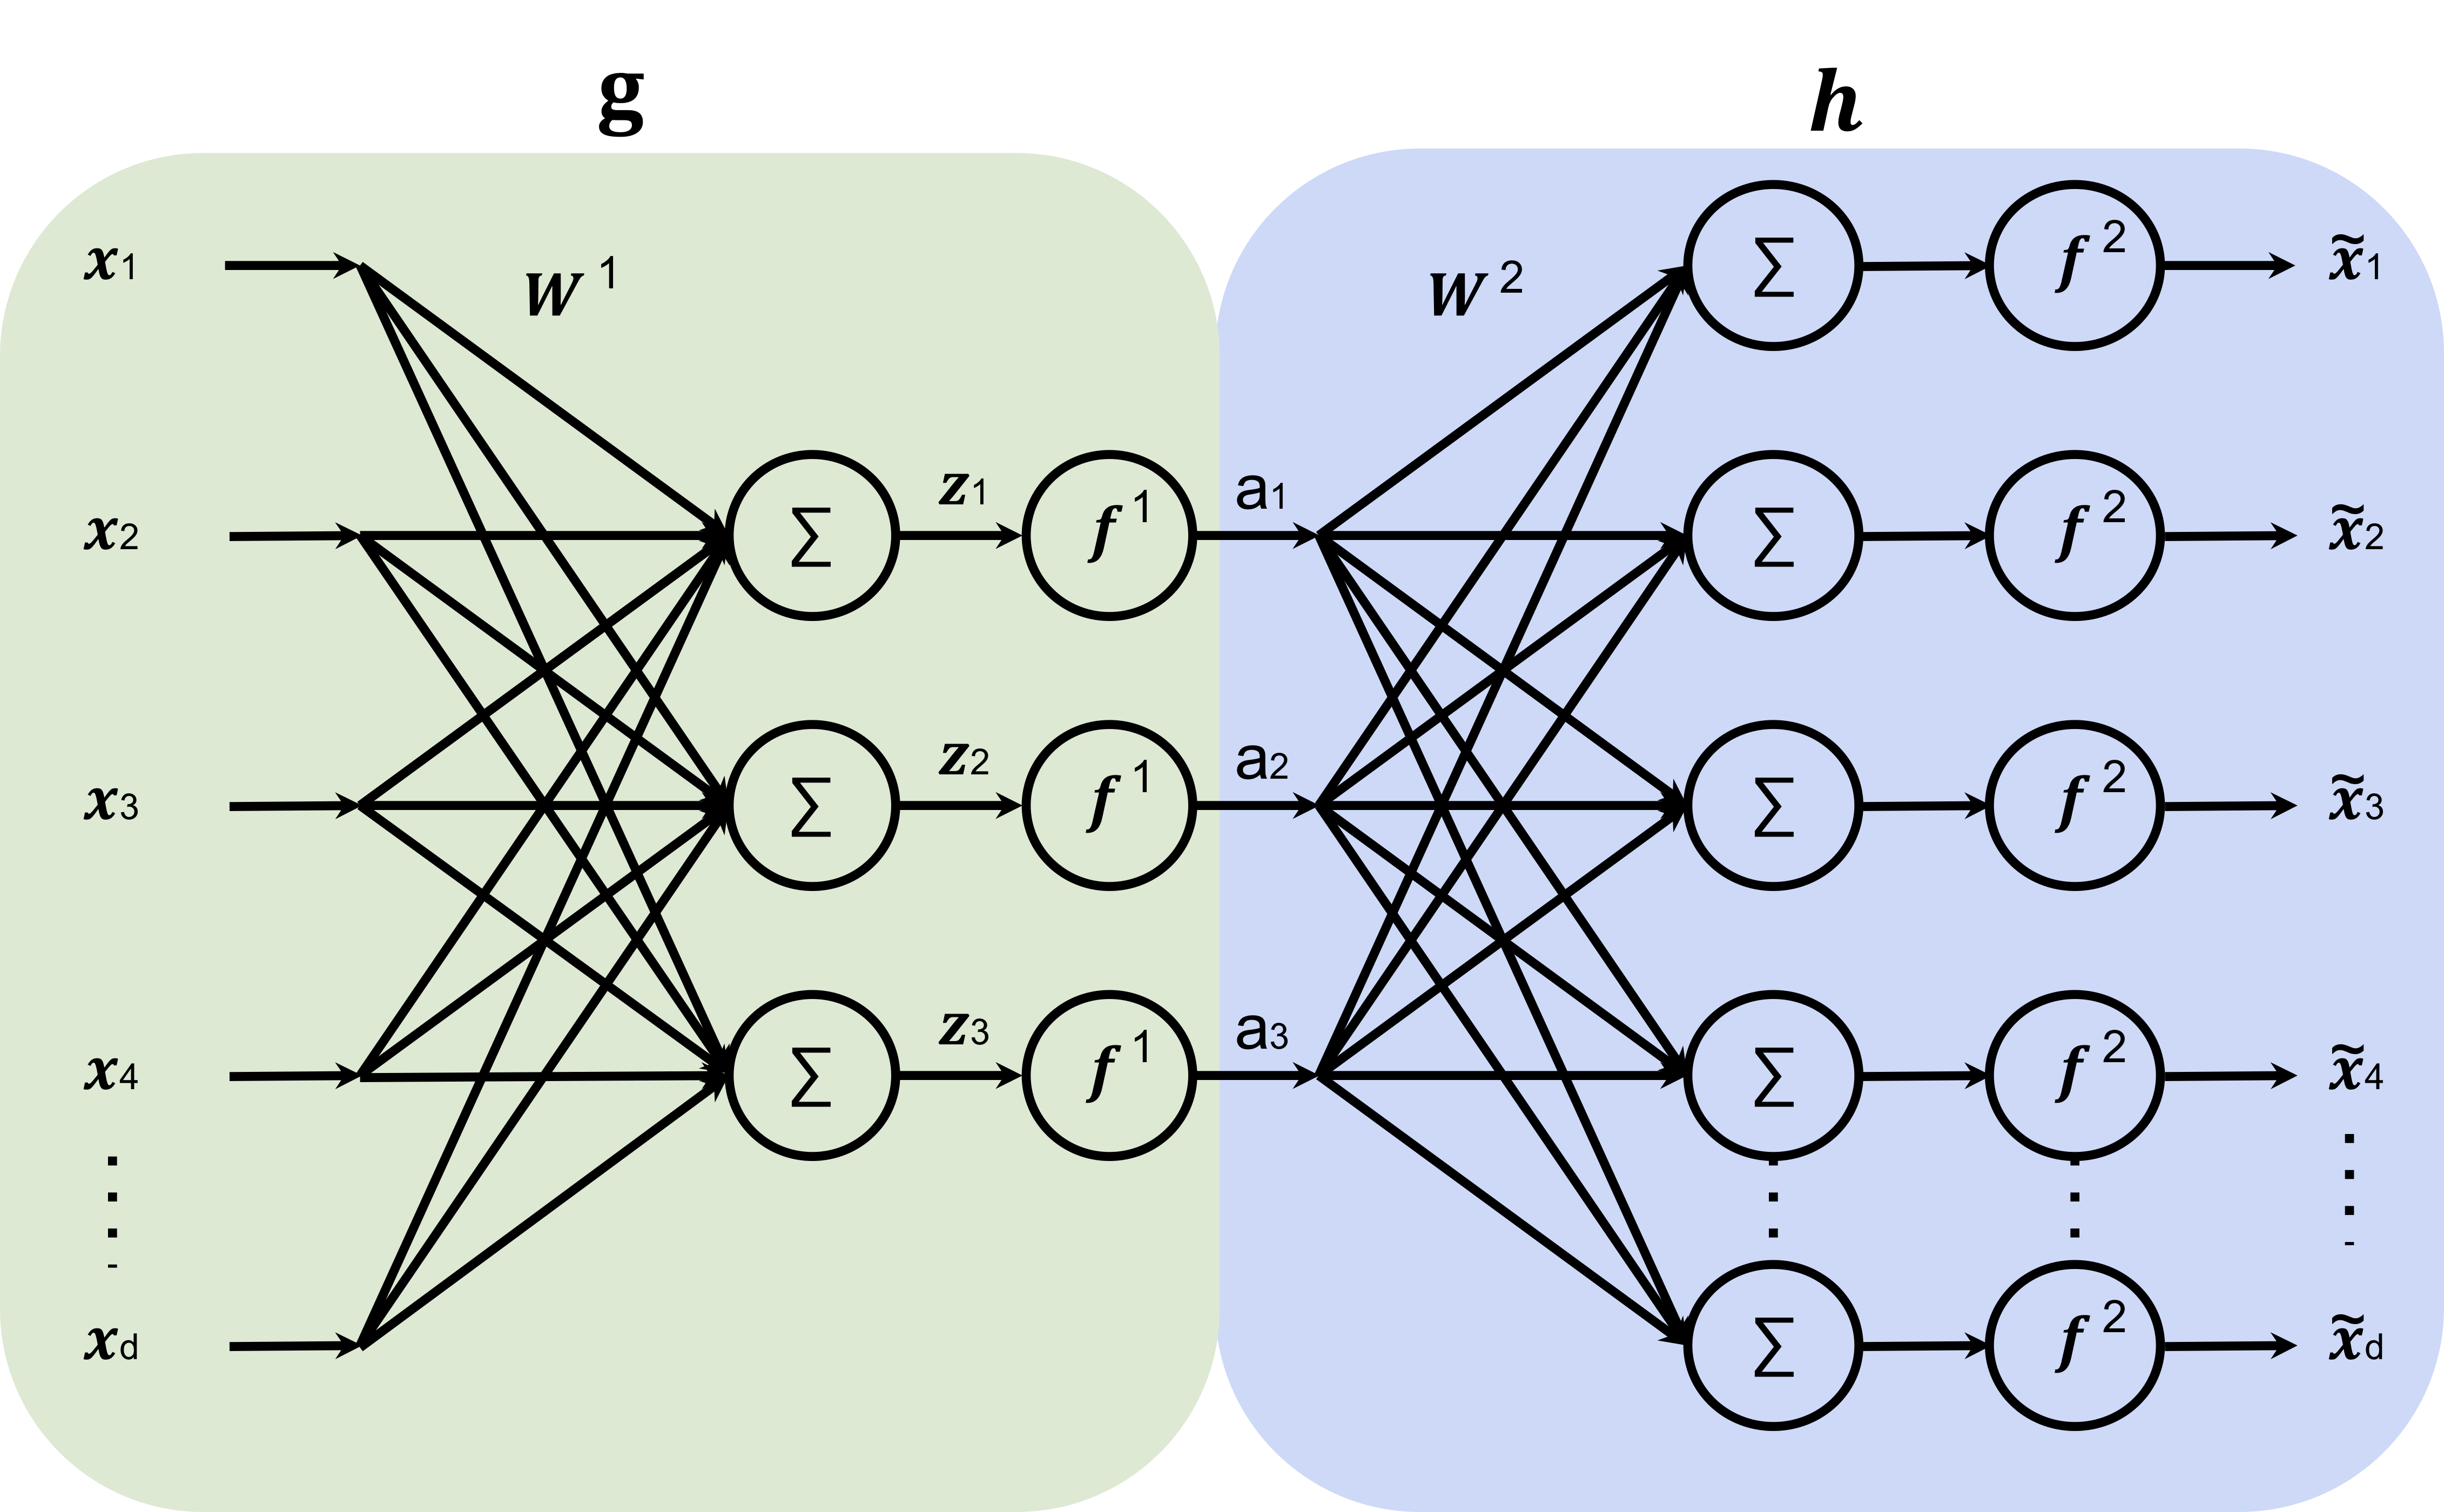
\includegraphics[width= .8\textwidth]{figures/autoencoder.png}
  \caption{\small Autoencoder structure, showing the encoder (left
    half, light green), and the decoder (right half, light blue),
    encoding inputs $x$ to the representation $a$, and decoding the
    representation to produce $\tilde{x}$, the reconstruction.  In
    this specific example, the representation ($a_1$, $a_2$, $a_3$)
    only has three dimensions.\label{fig:autoencoder}}
\end{figure}

\newpage
\section{Autoencoder Learning}

We learn the weights in an autoencoder using the same tools that we previously used for
supervised learning, namely (stochastic) gradient descent of a
multi-layer neural network to minimize a loss function. All that
remains is to specify the loss function $\mathcal{L}(\tilde{x}, x)$, which tells
us how to measure the discrepancy between the reconstruction
$\tilde{x} = h(g(x; W^{1}, W^1_0); W^{2}, W^2_0)$ and the original input $x$. For
example, for continuous-valued $x$ it might make sense to use squared
loss, i.e., $\mathcal{L}_{SE}(\tilde{x}, x) = \sum_{j=1}^{d} (x_j -
  \tilde{x}_j)^2$.\note{Alternatively, you could think of this as {\em
      multi-task learning}, where the goal is to predict each dimension
  of $x$. One can mix-and-match loss functions as appropriate for each
  dimension's data type.} Learning then seeks to optimize the
parameters of $h$ and $g$ so as to minimize the reconstruction error,
measured according to this loss function:
\[
  \min_{W^{1}, W^1_0, W^{2}, W^2_0} \sum_{i=1}^n \mathcal{L}_{SE}\left(h(g(x^{(i)}; W^{1}, W^1_0); W^{2}, W^2_0), x^{(i)}\right)
\]

\section{Evaluating an autoencoder}

What makes a good learned representation in an autoencoder? Notice
that, without further constraints, it is always possible to perfectly
reconstruct the input. For example, we could let $k=d$ and $h$ and $g$
be the identity functions. In this case, we would not obtain any
compression of the data.

To learn something useful, we must create a
\textit{bottleneck} by making $k$ to be smaller (often much smaller)
than $d$. This forces the learning algorithm to seek transformations
that describe the original data using as simple a description as
possible. Thinking back to the digits dataset, for example, an example
of a compressed representation might be the digit label (i.e., 0--9),
rotation, and stroke thickness. Of course, there is no guarantee that
the learning algorithm will discover precisely this
representation. After learning, we can inspect the learned
representations, such as by artificially increasing or decreasing one
of the dimensions (e.g., $a_1$) and seeing how it affects the output
$h(a)$, to try to better understand what it has learned.

As with clustering, autoencoders can be a preliminary step toward
building other models, such as a regressor or classifier. For example,
once a good encoder has been learned, the decoder might be replaced
with another neural network that is then trained with supervised learning
(perhaps using a smaller dataset that does include labels).

\section{Linear encoders and decoders}

We close by mentioning that even linear encoders and decoders can be
very powerful. In this case, rather than minimizing the above
objective with gradient descent, a technique called \textit{principal
  components analysis} (PCA) can be used to obtain a closed-form
solution to the optimization problem using a singular value
decomposition (SVD).  Just as a multilayer neural network with
nonlinear activations for regression (learned by gradient descent) can
be thought of as a nonlinear generalization of a linear regressor (fit
by matrix algebraic operations), the neural network based autoencoders
discussed above (and learned with gradient descent) can be thought of
as a generalization of linear PCA (as solved with matrix algebra by
SVD).

\section{Advanced encoders and decoders}

Advanced neural networks that build on the encoder-decoder conceptual
decomposition have become increasingly powerful in recent years. One
family of applications are {\em generative}\index{generative networks}
networks, where new outputs that are ``similar to'' but different from
any existing training sample are desired. In {\em variational
    autoencoders}\index{autoencoder!variational} the compressed
representation encompasses information about the probability
distribution of training samples, e.g., learning both mean and
standard deviation variables in the bottleneck layer or latent
representation. Then, new outputs can be generated by random sampling
based on the latent representation variables and feeding those samples
into the decoder.

  {\em Transformer} neural networks use {\em multiple} encoder and
decoder blocks, together with a self-attention mechanism to make predictions
about potential next outputs resulting from sequences of inputs. Such
transformer networks have many applications in natural language
processing and elsewhere. We will learn about sequential models in
Chapter~\ref{chap-rnn}.

